\documentclass[10pt]{beamer}
\usetheme{metropolis}  
\usecolortheme{beaver}
\usepackage{hyperref}
\usepackage{bigints}
\title{Introducci\'on a la probabilidad y estad\'istica CM274}
 \usepackage[spanish]{babel}
 \decimalpoint
\date{\today}
\author{C\'esar Lara Avila}
\institute{\url{https://github.com/C-Lara}}
\begin{document}
  \maketitle
  \section{3. Probabilidad condicional, eventos independientes
  	Regla de Bayes}
  
  
  \begin{frame}{Probabilidad condicional }
Asumiendo $P(B) > 0$, definimos la \underline{probabilidad condicional} de $A$, dado que $B$ a ocurrido como sigue, 

\[
\mathbb{P}(A|B ) = \frac{\mathbb{P}(A \cap B)}{\mathbb{P}(B)}
\]



Para cualquier evento $B$ fijo  tal que  $P (B)> 0, \mathbb{P} (\cdot| B)$ es una funci\'on de  probabilidad (es decir, que cumple los tres axiomas de probabilidad). 

En particular $\mathbb{P}(A|B) \geq 0, \mathbb{P}(\Omega|B) = 1$ y si $A_1,A_2, \dots $ son disjuntos, entonces $\mathbb{P}(\bigcup\limits_{i= 1}^{\infty}A_i|B)= \sum_{i = 1}^{\infty}\mathbb{P}(A_i|B)$. 

Pero no es cierto en general que $\mathbb{P}(A|B \cup C) = \mathbb{P}(A|B) + P(A|C)$.

\end{frame}

 \begin{frame}{Propiedades de la probabilidad condicional }
\small {Si $\mathbb{P}(A) > 0$ y $\mathbb{P}(B) > 0$, tenemos
 
 \[
 \mathbb{P}(A\cap B)=\mathbb{P}(A|B)\mathbb{P}(B)=\mathbb{P}(B|A)\mathbb{P}(A).
 \]
 
 \vspace{0.3cm}
 
 Intuitivamente, $\mathbb{P}(A | B)$ es la probabilidad de que $A$ ocurra suponiendo que ocurri\'o el evento $B$. De acuerdo con esa intuici\'on, la probabilidad condicional tiene las siguientes propiedades}
 
 \begin{itemize}
 	\item Si $B \subset A$ entonces $\mathbb{P}(A| B)=\mathbb{P}(B)/\mathbb{P}(B)=1$.
 	\item Si $A \cap B = \emptyset$ entonces $\mathbb{P}(A | B)=0/\mathbb{P}(B)=0$.
 	\item $A \subset B$ entonces $\mathbb{P}(A| B)=\mathbb{P}(A)/\mathbb{P}(B)$.
 	\item La probabilidad condicional, puede ser vista como una funci\'on de probabilidad
 	
 	\[
 	\mathbb{P}_A(E)  =  \mathbb{P}(E | A)
 	\]
 	y todas las propiedades y intuiciones que se aplican a la funci\'on probabilidad se aplican a $\mathbb{P}_A$ tambi\'en.
 \end{itemize}
\end{frame}
\begin{frame}{Ejemplo explicativo }
Observamos en la siguiente figura, que $\mathbb{P}(A \cap B) = 1/6$, que $\mathbb{P}(B) = 1/2$ y que $\mathbb{P}(A|B) = (1/6)/(1/2) = 1/3$, como se esperaba.

Sabemos que $B$ ha ocurrido y que el evento $A$ ocurrir\'a si uno de los cuatro resultados en $A \cap B$ se elige entre los $12$ igualmente probable.

\begin{figure}[h]
	\centering
	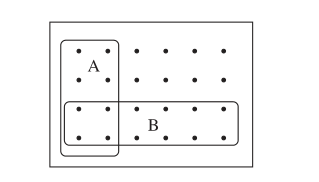
\includegraphics[width=6cm]{g1}
\end{figure}

\scriptsize{Podemos generalizar la ecuaci\'on de la probabilidad condicional a m\'ultiples eventos. Sea $A_i, i = 1,2, \dots, k$ para $k$ eventos para el cual $\mathbb{P}(A_1 \cap A_2 \cap \cdots A_k) > 0$. Entonces

\[
\mathbb{P}(A_1 \cap A_2 \cap \cdots A_k) = \mathbb{P}(A_1)\mathbb{P}(A_2|A_1)\mathbb{P}(A_3|A_1 \cap A_2)\cdots \mathbb{P}(A_k|A_1 \cap A_2 \cap \cdots \cap A_{k -1}).
\]
}
\end{frame}
\begin{frame}{Ejemplo contraintuitivo Feller 1968}
\small{Consideramos dos familias con dos hijos donde la probabilidad de g\'enero de cada ni\~no es sim\'etrica $(1/2)$. Seleccionamos una familia al azar y consideramos el espacio muestral que describe el g\'enero de los ni\~nos $\Omega=\{MM,MF,FM,FF\}$. Asumimos un modelo cl\'asico, implicando que las probabilidades de  todos los eventos elementales son $1/4$.
	
		
\vspace{0.2cm}	
		
Definimos el evento  en que ambos hijos en la familia son ni\~nos como $A=\{MM\}$, el evento que una familia tiene un ni\~no es $B=\{MF,FM,MM\}$ y el evento que el primer hijo es un ni\~no como $C=\{MF,MM\}$.
		
		
Dado que el primer hijo  es un ni\~no, la probabilidad de que ambos hijos sean ni\~nos es $\mathbb{P}(A | C)=\mathbb{P}(A\cap C)/\mathbb{P}(C)=\mathbb{P}(A)/\mathbb{P}(C)=(1/4)/(1/2)=1/2.$
		
		
\vspace{0.2cm}
		
Esto coincide con nuestra intuici\'on. Dado que la familia tiene un ni\~no, la probabilidad de que ambos hijos sean ni\~nos es contraintuitiva}
		
\[
\mathbb{P}(A| B)=\mathbb{P}(A\cap B)/\mathbb{P}(B)=\mathbb{P}(A)/\mathbb{P}(B)=(1/4)/(3/4)=1/3.
\]
\end{frame}


\begin{frame}{Independencia}

\small{Dos eventos  $A$ y $B$ son independientes si  $\mathbb{P}(A\cap B) = \mathbb{P}(A)\mathbb{P}(B)$.  Para tres eventos, $A, B$ y $C$ definimos los eventos independientes si
	
	\begin{align*}
	\mathbb{P}(A \cap B) &= \mathbb{P}(A)\mathbb{P}(B)\\
	\mathbb{P}(A \cap C) &= \mathbb{P}(A)\mathbb{P}(C)\\
	\mathbb{P}(B \cap C) &= \mathbb{P}(A)\mathbb{P}(C)\ \ \text{y} \\
	\mathbb{P}(A \cap B \cap C) &= \mathbb{P}(A)\mathbb{P}(B)\mathbb{P}(C).
	\end{align*}
	
	
Las tres primeras de estas condiciones establecen que los eventos son independientes dos a dos , por lo que llamamos a estos eventos que satisfacen estas tres condiciones como \underline{\texttt{independientes por pares}}. Para un n\'umero finito de eventos $A_1, A_2, \dots, A_n$ son independientes si
	
\[
\mathbb{P}(A_1\cap\cdots A_n)=\mathbb{P}(A_1)\cdots \mathbb{P}(A_n)
\]
	
y son independientes por pares si cada par $A_i, A_j,  i \neq j$ son independientes.}
\end{frame}

\begin{frame}{Generalizaci\'on del concepto }	
\small{Si generalizamos un poco, dado un conjunto  de eventos $\{ A_i: i \in I \}$ estos  son independientes si
	
\[
	\mathbb{P}\Bigl(  \bigcap\limits_{i \in J}A_i \Bigr)  = \prod_{i \in J}\mathbb{P}(A_i)  
\]
	
para cada subconjunto $J$ de $I$.

\vspace{0.2cm}


 M\'ultiples eventos $A_{\theta}, \theta \in \Theta$ son independientes por pares si cada par de eventos es independiente.  M\'ultiples eventos $A_{\theta}, \theta \in \Theta$ son independientes si para cada $k > 0$ y para cada k-subconjunto de distintos eventos $A_{\theta_1},\ldots,A_{\theta_k}$, tenemos}
	
	\[
	\mathbb{P}(A_{\theta_1}\cap\ldots\cap A_{\theta_k})=\mathbb{P}(A_{\theta_1})\cdots \mathbb{P}(A_{\theta})
	\]

\vspace{0.2cm}

\scriptsize{La anterior definici\'on generaliza la independencia de una colecci\'on arbitraria de eventos, indexados por un conjunto (potencialmente infinito) $\Theta$.}
\end{frame}

\begin{frame}{Contraejemplo explicativo}
\small{Una moneda es lanzada $4$ veces. Consideremos los eventos $A$ donde la primera moneda muestra cara; $B$ la tercera moneda muestra sello; y $C$ hay un n\'umero igual de caras y sellos. ?` Esos son eventos independientes ?.

Supongamos que el espacio muestral consiste de $16$ puntos que muestran los lanzamientos. 

\vspace{0.2cm}

Entonces $\mathbb{P}(A) = 1/2$ y $\mathbb{P}(B) = 1/2$, mientras que $C$ consiste de $6$ puntos con exactamente dos caras y dos sellos. As\'i $P(C) = 6/16 = 3/8$. Ahora $\mathbb{P}(A \cap B) =\frac{4}{16} = \frac{1}{4} = \mathbb{P}(A)\mathbb{P}(B); \mathbb{P}(A \cap C) = \frac{3}{16} = \mathbb{P}(A)\mathbb{P}(C)$ y $\mathbb{P}(B \cap C) = \frac{3}{16} =  \mathbb{P}(B)\mathbb{P}(C)$. Por tanto los eventos $A, B$ y $C$ son independientes por pares.

\vspace{0.2cm}

El evento $A \cap B \cap C$ consiste de dos puntos $CSSC$ y $CCSS$ con probabilidad $2/16 = 1/8$. As\'i $\mathbb{P}(A \cap B \cap C) \neq \mathbb{P}(A)\mathbb{P}(B)\mathbb{P}(B)$. Luego los evento $A, B$ y $C$ no son independientes.	}
\end{frame}
\begin{frame}{Ley de la probabilidad total }

Sea $A$ un evento, entonces se sabe que la intersecci\'on de $A$ y el evento universal $\Omega$ es $A$. Se sabe adem\'as que $B$ y su complemento $B^c$ constituye una partici\'on. As\'i

\[
A = A \cap \Omega \ \  \text{y}\ \  B \cup B^c = \Omega
\]

\vspace{0.2cm}

Sustituyendo el segundo resultado en el primero en la ecuaci\'on anterior y aplicando la Ley de Morgan, tenemos


\begin{equation*}
A = A \cap ( B \cup B^c) = (A \cap B) \cup (A \cap  B^c).
\end{equation*}

\end{frame}

\begin{frame}{Ley de la probabilidad total(1) }
Los eventos $(A \cap B)$ y  $ (A \cap B^c)$ son mutualmente exclusivos y de acuerdo al siguiente gr\'afico, 


\begin{figure}[h]
	\centering
	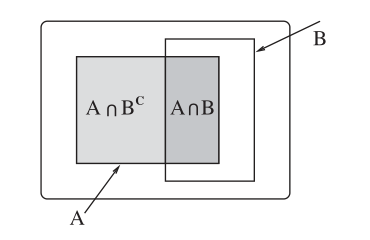
\includegraphics[width=6cm]{g2}
\end{figure}
Se muestra que $B$ y $B^c$ no pueden tener salidas en com\'un, la intersecci\'on de $A$ y $B$ no puede tener salidas en com\'un con la intersecci\'on de $A$ y $B^c$,	
\end{frame}

\begin{frame}{Ley de la probabilidad total(2)}
Usando el hecho que  $(A \cap B)$ y  $ (A \cap B^c)$ son mutualmente exclusivos y por propiedad de la funci\'on probabilidad, se tiene

\vspace{0.2cm}

\[
\mathbb{P}(A) = \mathbb{P}(A \cap B) + \mathbb{P}(A \cap B^c).
\]


Esto significa que para evaluar la probabilidad de un evento $A$, es suficiente encontrar las probabilidades de la intersecci\'on de $A$ y $B$ y $A$ y $B^c$ y sumarlos. 



En general sean $n$ eventos $B_i, i = 1, 2, \dots, n$, una partici\'on del espacio muestral $\Omega$. Entonces para alg\'un evento $A$, podemos escribir


\[
\mathbb{P}(A) = \sum_{i  =1}^n \mathbb{P}(A \cap B_i), \ \  n \geq 1
\]

Esta es la \underline{ley  de la probabilidad total}.
\end{frame}

\begin{frame}{Ley de la probabilidad total(3)}
	
En efecto, los conjuntos $A \cap B_i, i = 1,2, \dots, n$ son mutualmente exclusivos (desde que los $B_i$ lo son) y el hecho que $B_i, i = 1,2, \dots$ es una partici\'on de $\Omega$ implica que

\[
A = \bigcup_{i =1}^{n}A \cap B_i,\ n \geq 1,
\]

y por propiedad de la funci\'on probabilidad (tercer axioma), se tiene

\vspace{0.2cm}

\[
\mathbb{P}(A) = \mathbb{P}\Biggl\{ \bigcup_{i = 1}^n A \cap B_i \Biggr\} = \sum_{i =1}^{n}\mathbb{P}(A \cap B_i).
\]

\end{frame}

\begin{frame}{Ejemplo explicativo}
\small{Consideramos la siguiente figura que muestra una partici\'on de un espacio muestral conteniendo $24$ equiprobables salidas en seis eventos $B_1$ hasta $B_6$.}
 
 \begin{figure}[h]
 	\centering
 	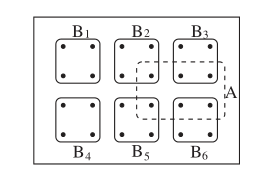
\includegraphics[width=5cm]{g3}
 \end{figure}
 
\vspace{0.3cm}

\scriptsize{Se sigue entonces que la probabilidad del evento $A$ es igual a $1/4$ ya que contiene seis de los puntos de muestreo. Debido a que los eventos $B_i$ constituyen una partici\'on, cada punto de $A$ est\'a en uno y s\'olo uno de los eventos $B_i$ y la probabilidad del evento $A$ se pueden encontrar sumando las probabilidades de los eventos $A \cap B_i$ para $i = 1,2, \dots,6$ . Para este ejemplo particular se puede ver que estas seis probabilidades est\'an dadas por $0, 1/24, 1/12, 0, 1/24$  y $1/12$ que cuando se suman juntas da 1/4.}

\end{frame}

\begin{frame}{Uso de \'arboles para organizar el c\'alculo}
\small{Los \'arboles son una  manera de organizar c\'alculos con probabilidad condicional y la ley de probabilidad total. Las figuras y los ejemplos muestran  lo que queremos decir con un \'arbol. Al igual que con la regla del producto, la clave es organizar el proceso subyacente en una secuencia de acciones.

\vspace{0.2cm}

Sea el siguiente \underline{ejemplo:} Una urna contiene 5 pelotas rojas y 2 pelotas gris. Se saca una pelota. Si es gris, se agrega una pelota roja a la urna y si es roja, se agrega una pelota gris a la urna. (La pelota original no se devuelve a la urna.) Luego se saca una segunda pelota. ?`Cu\'al es la probabilidad de que la segunda pelota sea roja?.

\vspace{0.2cm}

Comenzamos rehaciendo el ejemplo anterior. La secuencia de acciones es: primero se saca  la pelota 1 (y a\~nade la bola apropiada a la urna) y luego se saca  la pelota 2.}
\end{frame}

\begin{frame}{Uso de \'arboles para organizar el c\'alculo(1)}
Sea el siguiente diagrama de \'arbol del ejemplo anterior:

\begin{figure}[h]
	\centering
	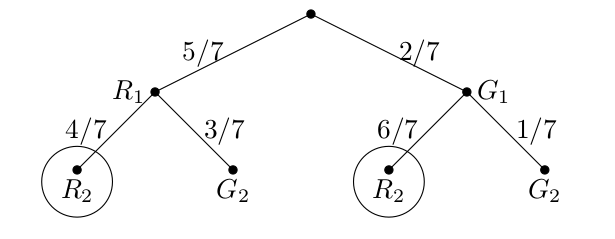
\includegraphics[width=7cm]{g4}
\end{figure}

\scriptsize{Se interpreta este \'arbol de la siguiente manera. Cada punto se llama \textcolor{blue}{nodo}. El \'arbol est\'a organizado por niveles. El nodo superior (nodo ra\'iz) est\'a en el nivel $0$. La capa siguiente es el nivel $1$ y as\'i sucesivamente. Cada nivel muestra los resultados en una etapa de la extracci\'on. El nivel $1$ muestra los posibles resultados de la primera extracci\'on. El nivel $2$ muestra los posibles resultados de la segunda extracci\'on   a partir de cada nodo en el nivel $1$.

\vspace{0.2cm}

Las probabilidades se escriben a lo largo de las ramas. La probabilidad de que $R_1$ (rojo en la primera extracci\'on ) es $5/7$. Esto se  escribe a lo largo de la rama desde el nodo de ra\'iz a un nodo  etiquetada por  $R_1$. En el siguiente nivel ponemos probabilidades condicionales. La probabilidad a lo largo de la rama de $R_1$ a $R_2$ es $\mathbb{P}(R_2|R_1) = 4/7$ que representa la probabilidad de ir al nodo $R_2$ dado que ya se est\'a en $R_1$.}
\end{frame}

\begin{frame}{Uso de \'arboles para organizar el c\'alculo(2)}
\small{La regla de multiplicaci\'on dice que la probabilidad de llegar a cualquier nodo es s\'olo el producto de las probabilidades a lo largo de la ruta  para llegar all\'i. Por ejemplo, el nodo etiquetado $R_2$ en la extrema izquierdo representa realmente el evento $R_1 \cap R _2$ porque proviene del nodo $R_1$. La regla de multiplicaci\'on dice:
	
	
\[
\mathbb{P}(R_1 \cap R _2) = \mathbb{P}(R_1)\mathbb{P}(R_2|R_1 ) = \frac{5}{7}\cdot\frac{4}{7},
\]	

que  se est\'a multiplicando exactamente a lo largo de la ruta  hacia el nodo.

\vspace{0.2cm}

La ley de probabilidad total es simplemente la afirmaci\'on de que $\mathbb{P}(R_2)$ es la suma de las probabilidades de todos las rutas  que conducen a $R_2$ (los dos nodos en c\'irculo en la figura). En este caso,

\[
\mathbb{P}(R_2) = \frac{5}{7}\times \frac{4}{7} + \frac{2}{7}\times\frac{6}{7} = \frac{32}{49}.
\]
}
\end{frame}

\begin{frame}{\'Arboles precisos}
El \'arbol anterior  implica ciertas simplificaciones. Por ejemplo, el nodo  $R_2$ en el extremo izquierdo representa realmente el evento $R_1 \cap R_2$, ya que termina en la ruta, desde la ra\'iz hasta $R_1$ hasta $R_2$.

Aqu\'i est\'a el mismo \'arbol  etiquetado con precisi\'on. 


\begin{figure}[h]
	\centering
	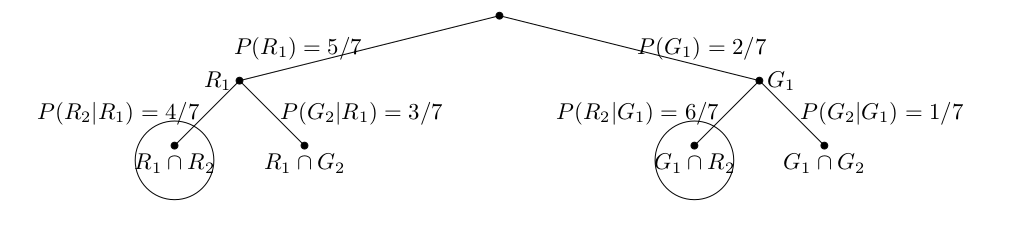
\includegraphics[width=11cm]{g6}
\end{figure}



Como se puede ver este \'arbol es m\'as complicado de hacer y de usar. Usualmente se usa una versi\'on  abreviada de los \'arboles.
\end{frame}

\begin{frame}{El teorema  de Bayes}
	
\small{El \underline{teorema de Bayes} es un pilar de la probabilidad y estad\'istica y es central para el resto de este curso y otros cursos m\'as avanzados . Para dos eventos $A$ y $B$ el teorema de Bayes (tambi\'en llamado la \underline{regla de Bayes} y \underline{f\'ormula de Bayes}) dice,

\[
\mathbb{P}(B|A) = \frac{\mathbb{P}(A|B)\mathbb{P}(B)}{\mathbb{P}(A)}.
\]

\begin{itemize}
	\item La regla de Bayes nos dice c\'omo invertir las probabilidades condicionales, es decir, encontrar $\mathbb{P}(B | A)$ de $\mathbb{P}(A | B)$.
\item En la pr\'actica, $\mathbb{P}(A)$ a menudo se calcula utilizando la ley de probabilidad total.

\end{itemize}
En efecto, obtenemos la regla de Bayes de resultados anteriores sobre la probabilidad condicional y el teorema de la probabilidad total. As\'i tenemos

\[
\mathbb{P}(B_j|A) = \frac{\mathbb{P}(A \cap B_j)}{\mathbb{P}(A)} = \frac{\mathbb{P}(A|B_j)\mathbb{P}(B_j)}{\sum_{i}\mathbb{P}(A|B_i)\mathbb{P}(B_i)}
\]
}
\end{frame}

\begin{frame}{Ejemplo explicativo}
\small{Considere una prueba de rutina de detecci\'on de una enfermedad. Supongamos que la frecuencia de la enfermedad en la poblaci\'on (tasa b\'asica) es del $0,5\%$. La prueba es muy precisa con un $5\%$ de tasa de falsos positivos y un $10\%$ de tasa de falsos negativos. Si se  toma la prueba y es  positivo. ?`Cu\'al es la probabilidad de que se tenga la enfermedad?
	
Haremos el c\'alculo tres veces: usando \underline{\'arboles}, \underline{tablas} y \underline{s\'imbolos}. Utilizamos la siguiente notaci\'on para los eventos relevantes:

\begin{itemize}
\item $D+$ = 'tienes la enfermedad'.
\item $D-$ = 'no tienes la enfermedad'.
\item $T+$ = 'prueba positiva'
\item $T-$ = 'prueba negativa'.
\end{itemize}

Se nos da $\mathbb{P}(D +) = 0.005$ y por lo tanto $\mathbb{P}(D-) = 0.995$. Las tasas falsas positivas y falsas negativas son (por definici\'on) probabilidades condicionales.
}
\end{frame}

\begin{frame}{Ejemplo explicativo (1)}
\small{	
\[
\mathbb{P}(\text{falso positivo}) = \mathbb{P}(T+|D-) = 0.05\quad \text{y}\quad \mathbb{P}(\text{falso negativo}) = \mathbb{P}(T-|D+) = 0.1.
\]
		
Las probabilidades complementarias se conocen como las  tasas negativas y  positivas verdaderas:
\[
\mathbb{P}(T-|D-) = 1 - \mathbb{P}(T+|D-) = 0.95 \quad \text{y}\quad   \mathbb{P}(T+|D+) = 1 - \mathbb{P}(T-|D+) = 0.9.
\]	
}
\underline{\textbf{\'Arboles:}}Todas estas probabilidades se pueden mostrar muy bien en un \'arbol.

\begin{figure}[h]
	\centering
	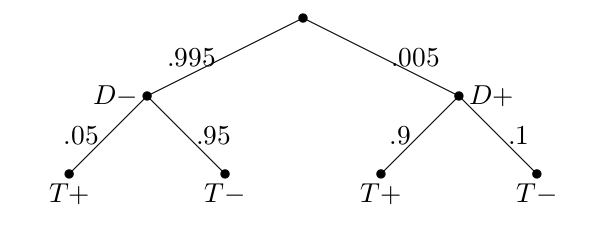
\includegraphics[width=6cm]{g7}
\end{figure}
La pregunta pide la probabilidad de que una persona tenga la enfermedad dado que  di\'o positivo, es decir, cu\'al es el valor de $\mathbb{P}(D+ | T +)$.
\end{frame}
\begin{frame}{Ejemplo explicativo (2)}
\small{ No se nos da este valor, pero si sabemos $\mathbb{P}(T+|D +)$, por lo que podemos usar el teorema de Bayes:

\[
\mathbb{P}(D+|T +) = \frac{\mathbb{P}(T+|D +)\cdot \mathbb{P}(D+ )}{\mathbb{P}(T+)}.
\]

Se dan las dos probabilidades en el numerador. Calculamos el denominador $\mathbb{P}(T +)$ utilizando la ley de probabilidad total. Usando el \'arbol s\'olo tenemos que sumar las probabilidades para cada uno de los nodos marcados con $T+$.

\[
\mathbb{P}(T +) = 0.995 \times 0.05 + 0.005 \times  0.9 = 0.05425
\]

As\'i,

\[
\mathbb{P}(D+|T +) = \frac{0.9 \times 0.005}{0.5425} = 0.082949 \approx 8.3\%.
\]	
}
\end{frame}
\begin{frame}{Ejemplo explicativo (3)}
\small\underline{\textbf{Tablas :}}{ Otro truco que es \'util para calcular las probabilidades es hacer una tabla. Vamos a repetir el ejemplo anterior usando una tabla construida con $10000$ personas totales divididas de acuerdo con las probabilidades en este ejemplo.

Construimos la tabla como sigue. Elegimos un n\'umero, digamos $10000$ personas  y colocamos  como el total general en la parte inferior derecha. Usando $\mathbb{P}(D +) = 0.005$ calculamos que $50$ de las $10000$ personas est\'an enfermas ($D+$). Del mismo modo $9950$ personas son saludables ($D-$). En este punto, la tabla se ve as\'i:

\begin{figure}[h]
	\centering
	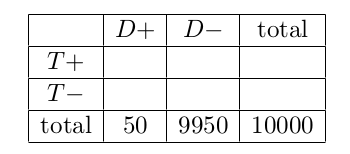
\includegraphics[width=4.5cm]{g8}
\end{figure}

Usando $P(T+|D +) = 0.9$ podemos calcular que el n\'umero de personas enfermas que dieron positivo en el $90\%$ de $50$ o $45$.
}
\end{frame}

\begin{frame}{Ejemplo explicativo (4)}
\small{Las otras entradas son similares. En este punto la tabla se parece a la tabla de abajo a la izquierda. Finalmente sumamos las filas $T+$ y $T-$ para obtener la tabla completa a la derecha.

\begin{figure}[h]
	\centering
	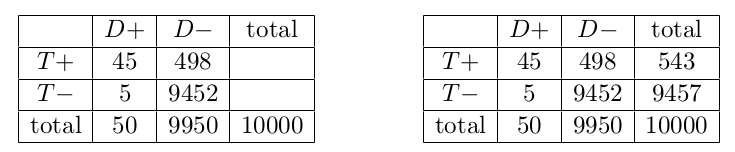
\includegraphics[width=8.5cm]{g9}
\end{figure}

Usando la tabla completa podemos calcular:

\[
\mathbb{P}(D+|T +) = \frac{\vert D+ \cap T+\vert }{\vert T+ \vert} = \frac{45}{543} = 8.3\%.
\]
}
\end{frame}
\begin{frame}{Ejemplo explicativo (5)}
\small\underline{\textbf{S\'imbolos:}}{ Para completar, mostramos c\'omo se ve la soluci\'on cuando se escribe directamente en s\'imbolos

\begin{align*}
\mathbb{P}(D+|T +)  &=  \frac{\mathbb{P}(T+|D +)\cdot \mathbb{P}(D+ )}{\mathbb{P}(T+)} \\
					&= \frac{\mathbb{P}(T+|D +)\cdot \mathbb{P}(D+ )}{\mathbb{P}(T+|D+)\mathbb{P}(D+)+ \mathbb{P}(T+|D-)\mathbb{P}(D-)}\\
					&= \frac{0.9 \times 0.005}{0.9 \times 0.005 + 0.05 \times 0.995}\\
					&= 8.3\%
\end{align*}	
}

\scriptsize{Esto se llama la falacia de la tasa de base porque la tasa de base de la enfermedad en la poblaci\'on es tan baja que la gran mayor\'ia de las personas que toman la prueba son saludables, e incluso con una prueba precisa la mayor\'ia de los positivos ser\'an personas sanas.}	
\end{frame}

\begin{frame}{Visualizaci\'on}
\small{La siguiente figura ilustra la falacia de la tasa de base. 
	
El \'area azul grande representa a toda la gente sana. El \'area roja mucho m\'as peque\~na representa a los enfermos. El rect\'angulo sombreado representa a la gente que prueba positivo. El \'area sombreada cubre la mayor parte de la zona roja y s\'olo una peque\~na parte de la zona azul. A\'un as\'i, la mayor parte del \'area sombreada est\'a sobre azul. Es decir, la mayoria de las pruebas positivas son de personas sanas.
	
\begin{figure}[h]
	\centering
	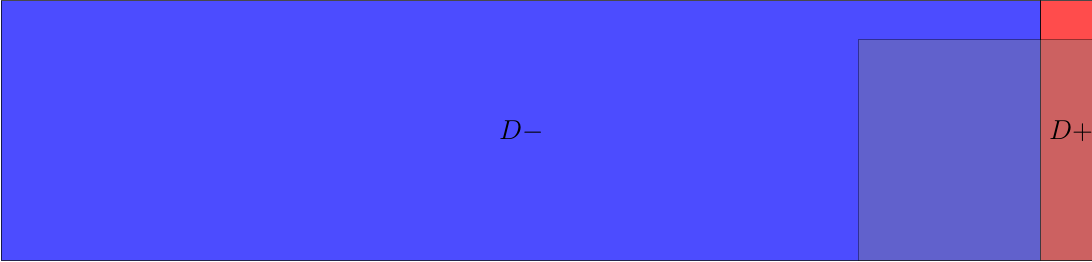
\includegraphics[width=8.5cm]{g10}
\end{figure}
}	

\scriptsize{\textcolor{blue}{Lectura:} Chapter 1 Probability Probability, Markov Chains, Queues and Simulation Willian J.Stewart Princeton University Press 2009.}
\end{frame}
\end{document}